%package list
\documentclass{article}
\usepackage[top=3cm, bottom=3cm, outer=3cm, inner=3cm]{geometry}
\usepackage{multicol}
\usepackage{graphicx}
\usepackage{url}
%\usepackage{cite}
\usepackage{hyperref}
\usepackage{array}
%\usepackage{multicol}
\newcolumntype{x}[1]{>{\centering\arraybackslash\hspace{0pt}}p{#1}}
\usepackage{natbib}
\usepackage{pdfpages}
\usepackage{multirow}
\usepackage[normalem]{ulem}
\useunder{\uline}{\ul}{}
\usepackage{svg}
\usepackage{xcolor}
\usepackage{listings}
\lstdefinestyle{ascii-tree}{
    literate={├}{|}1 {─}{--}1 {└}{+}1 
  }
\lstset{basicstyle=\ttfamily,
  showstringspaces=false,
  commentstyle=\color{red},
  keywordstyle=\color{blue}
}
\lstset{basicstyle=\ttfamily\fontfamily{Consolas}\selectfont,
	showstringspaces=false,
	commentstyle=\color{red},
	keywordstyle=\color{blue},
	literate={á}{{\'a}}1 {é}{{\'e}}1 {í}{{\'i}}1 {ó}{{\'o}}1 {ú}{{\'u}}1 {ñ}{{\~n}}1 {Á}{{\'A}}1 {É}{{\'E}}1 {Í}{{\'I}}1 {Ó}{{\'O}}1 {Ú}{{\'U}}1 {ñ}{{\~n}}1 {Ñ}{{\~N}}1 {ü}{{\"u}}1 {Ü}{{\"U}}1 {¡}{{!`}}1 {¿}{{?`}}1
}
%\usepackage{booktabs}
\usepackage{caption}
\usepackage{subcaption}
\usepackage{float}
\usepackage{array}

\newcolumntype{M}[1]{>{\centering\arraybackslash}m{#1}}
\newcolumntype{N}{@{}m{0pt}@{}}


%%%%%%%%%%%%%%%%%%%%%%%%%%%%%%%%%%%%%%%%%%%%%%%%%%%%%%%%%%%%%%%%%%%%%%%%%%%%
%%%%%%%%%%%%%%%%%%%%%%%%%%%%%%%%%%%%%%%%%%%%%%%%%%%%%%%%%%%%%%%%%%%%%%%%%%%%
\newcommand{\itemEmail}{jcondorios@unsa.edu.pe \par jcusilaymeg@unsa.edu.pe \par almamanima@unsa.edu.pe \par cvaldivialu@unsa.edu.pe}
\newcommand{\itemStudent}{Condorios Yllapuma Jorge \par Cusilayme García José Luis \par Mamani Mamani Alexis \par Valdivia Luna Carlo Joaquín}
\newcommand{\itemProffesor}{Richart Smith Escobedo Quispe}
\newcommand{\itemProffEmail}{rescobedoq@unsa.edu.pe}
\newcommand{\itemCourse}{Estructura de Datos}
\newcommand{\itemCourseCode}{20222076 \par 20220598 \par 20222066  \par 20220567}
\newcommand{\itemSemester}{III}
\newcommand{\itemUniversity}{Universidad Nacional de San Agustín de Arequipa}
\newcommand{\itemFaculty}{Facultad de Ingeniería de Producción y Servicios}
\newcommand{\itemDepartment}{Departamento Académico de Ingeniería de Sistemas e Informática}
\newcommand{\itemSchool}{Escuela Profesional de Ingeniería de Sistemas}
\newcommand{\itemAcademic}{2023 - A}
\newcommand{\itemInput}{Del 19 Julio 2023}
\newcommand{\itemOutput}{Al 23 Julio 2023}
\newcommand{\itemPracticeNumber}{06}
\newcommand{\itemTheme}{Tries}
%%%%%%%%%%%%%%%%%%%%%%%%%%%%%%%%%%%%%%%%%%%%%%%%%%%%%%%%%%%%%%%%%%%%%%%%%%%%
%%%%%%%%%%%%%%%%%%%%%%%%%%%%%%%%%%%%%%%%%%%%%%%%%%%%%%%%%%%%%%%%%%%%%%%%%%%%

\usepackage[english,spanish]{babel}
\usepackage[utf8]{inputenc}
\AtBeginDocument{\selectlanguage{spanish}}
\renewcommand{\figurename}{Figura}
\renewcommand{\refname}{Referencias}
\renewcommand{\tablename}{Tabla} %esto no funciona cuando se usa babel
\AtBeginDocument{%
	\renewcommand\tablename{Tabla}
}

\usepackage{fancyhdr}
\pagestyle{fancy}
\fancyhf{}
\setlength{\headheight}{30pt}
\renewcommand{\headrulewidth}{1pt}
\renewcommand{\footrulewidth}{1pt}
\fancyhead[L]{\raisebox{-0.2\height}{
\includegraphics[width=3cm]{img/logo_episunsa.png}}}
\fancyhead[C]{\fontsize{7}{7}\selectfont	\itemUniversity \\ \itemFaculty \\ \itemDepartment \\ \itemSchool \\ \textbf{\itemCourse}}
\fancyhead[R]{\raisebox{-0.2\height}{
\includegraphics[width=1.2cm]{img/logo_abet}}}
\fancyfoot[L]{Grupo EDA}
\fancyfoot[C]{\itemCourse}
\fancyfoot[R]{Página \thepage}

% para el codigo fuente
\usepackage{listings}
\usepackage{color, colortbl}
\definecolor{dkgreen}{rgb}{0,0.6,0}
\definecolor{gray}{rgb}{0.5,0.5,0.5}
\definecolor{mauve}{rgb}{0.58,0,0.82}
\definecolor{codebackground}{rgb}{0.95, 0.95, 0.92}
\definecolor{tablebackground}{rgb}{0.8, 0, 0}

\lstset{frame=tb,
	language=bash,
	aboveskip=3mm,
	belowskip=3mm,
	showstringspaces=false,
	columns=flexible,
	basicstyle={\small\ttfamily},
	numbers=none,
	numberstyle=\tiny\color{gray},
	keywordstyle=\color{blue},
	commentstyle=\color{dkgreen},
	stringstyle=\color{mauve},
	breaklines=true,
	breakatwhitespace=true,
	tabsize=3,
	backgroundcolor= \color{codebackground},
}

\begin{document}
	
	\vspace*{10px}
	
	\begin{center}	
		\fontsize{17}{17} \textbf{ Informe de Laboratorio \itemPracticeNumber}
	\end{center}
	\centerline{\textbf{\Large Tema: \itemTheme}}
	%\vspace*{0.5cm}	

	\begin{flushright}
		\begin{tabular}{|M{2.5cm}|N|}
			\hline 
			\rowcolor{tablebackground}
			\color{white} \textbf{Nota}  \\
			\hline 
			     \\[30pt]
			\hline 			
		\end{tabular}
	\end{flushright}	

	\begin{table}[H]
		\begin{tabular}{|x{4.7cm}|x{4.8cm}|x{4.8cm}|}
			\hline 
			\rowcolor{tablebackground}
			\color{white} \textbf{Estudiante} & \color{white}\textbf{CUI}  & \color{white}\textbf{Correo} \\
			\hline 
			{\itemStudent} & {\itemCourseCode} & {\itemEmail }     \\
			\hline 			
		\end{tabular}
	\end{table}		
	
	\begin{table}[H]
		\begin{tabular}{|x{4.7cm}|x{4.8cm}|x{4.8cm}|}
			\hline 
			\rowcolor{tablebackground}
			\color{white} \textbf{Facultad} & \color{white}\textbf{Asignatura}  & \color{white}\textbf{Docente}\\
			\hline 
			{\itemSchool} & {\itemCourse \par Semestre: \itemSemester}   & {\itemProffesor \par \itemProffEmail} \\
			\hline 			
		\end{tabular}
	\end{table}	
	
	\begin{table}[H]
		\begin{tabular}{|x{4.7cm}|x{4.8cm}|x{4.8cm}|}
			\hline 
			\rowcolor{tablebackground}
			\color{white}\textbf{Laboratorio} & \color{white}\textbf{Tema}  & \color{white}\textbf{Duración}   \\
			\hline 
			\itemPracticeNumber & \itemTheme & 02 horas   \\
			\hline 
		\end{tabular}
	\end{table}
	
	\begin{table}[H]
		\begin{tabular}{|x{4.7cm}|x{4.8cm}|x{4.8cm}|}
			\hline 
			\rowcolor{tablebackground}
			\color{white}\textbf{Semestre académico} & \color{white}\textbf{Fecha de inicio}  & \color{white}\textbf{Fecha de entrega}   \\
			\hline 
			\itemAcademic & \itemInput &  \itemOutput  \\
			\hline 
		\end{tabular}
	\end{table}
	
	\section{Tarea}
	\begin{itemize}		
		\item Elabore un informe paso a paso de la implementación una Trie para insertar, buscar y reemplazar palabras en un texto.
		\item Utilice interfaces gráficas de usuario para su implementación.
		\item Utilice todas las recomendaciones dadas por el docente.
		\item Utilice la siguiente GUI como referencia:
		
	\end{itemize}
		 
		
	\section{Equipos, materiales y temas utilizados}
	\begin{itemize}
		\item Sistema Operativo Windows 10 Home 64 bits (10.0, compilation 19045)
		\item VIM 9.0.
		\item OpenJDK 64-Bits 17.0.7.
		\item Git 2.39.2.
		\item Cuenta en GitHub con el correo institucional.
		\item Java 
	\end{itemize}
	
	\section{URL de Repositorio Github}
	\begin{itemize}
		\item URL del Repositorio GitHub para clonar o recuperar.
		\item \url{https://github.com/JorgeCY21/EDA_LAB_D}
		\item URL para el laboratorio 06 en el Repositorio GitHub.
		\item \url{https://github.com/JorgeCY21/EDA_LAB_D/tree/main/Lab_06}
	\end{itemize}
	
	\section{Actividades con el repositorio GitHub}
	
	\subsection{Creando e inicializando repositorio GitHub}
	\begin{itemize}
		\item Se realizaron los siguientes comandos en la computadora:
	\end{itemize}	
		
	\begin{lstlisting}[language=bash,caption={Dirijíéndonos al directorio de trabajo}][H]
		D:\
	\end{lstlisting}	
	\begin{lstlisting}[language=bash,caption={Clonando repositorio GitHub}][H]
		D:\ git clone https://github.com/JorgeCY21/EDA_LAB_D
	\end{lstlisting}
	\begin{lstlisting}[language=bash,caption={Inicializando directorio para laboratorio 06}][H]
		D:\ cd EDA_LAB_D
      D: \EDA_LAB_D> mkdir lab06
		D: \EDA_LAB_D> cd lab06
	\end{lstlisting}
	
	\subsection{Commits}
	\begin{lstlisting}[language=bash,caption={Commit: Creamos el trie principal}][H]
		
		D: \EDA_LAB_D\Lab_06> git add .
		D: \EDA_LAB_D\Lab_06> git commit -m "Creando entorno principal de trie"	
		D: \EDA_LAB_D\Lab_06> git push -u origin main
	\end{lstlisting}
 
	
	\section{Códigos Fuente}	
	\begin{minipage}{\textwidth}	

		\textbf{TrieNode: }
		\lstinputlisting[language=java, caption={TrieNode}]{src/TrieNode.java}
		En el primer fragmento de código se representa la clase TrieNode, el cual contiene un arreglo
		de 255 elementos(estos representan el código ACCII). Observamos dos atributos. El primero
		nos ayudará para conocer a al nodo siguiente, es decir, ayudara a la conexión con otros nodos para
		representar palabras completas o prefijos. Y el segundo atributo nos ayuda a saber si es el final de la palabra.

	\end{minipage}

	\begin{minipage}{\textwidth}	

		\textbf{Trie: }
		\lstinputlisting[language=java, caption={Trie-insertar}, linerange={1-27}]{src/Trie.java}
		En la primera sección del código Trie observamos Nodo raíz de nuestro Trie, despues dos constructores, 
		el segundo constructor pide como parámetro texto el cual primero al texto lo dividiremos en palabras, 
		esto haremos mediante la expresión regular "\textbackslash\textbackslash s+" para después con un foreach insertar las palabras en nuestro trie
		\\El método para insertar una palabra en el Trie. Comienza desde el nodo raíz y recorre cada carácter de la palabra. 
		Si el carácter no tiene un nodo hijo, se crea un nuevo nodo. Luego, se mueve al siguiente nodo hijo correspondiente al 
		siguiente carácter. Al final de la palabra, marca el último nodo como un nodo de fin de palabra \(setIsEndWord(true)\) 
		para indicar que se ha insertado una palabra completa.
		
		\end{minipage}
		\clearpage
		\lstinputlisting[language=java, caption={Trie-eliminación}, linerange={29-53}]{src/Trie.java}
		El método recorre el Trie buscando el camino hacia la palabra a eliminar, almacenando los nodos visitados en el camino en un arreglo llamado parents. 
		Si la palabra no existe en el Trie (es decir, no se encuentra el último nodo correspondiente al último carácter de la palabra), el método simplemente 
		retorna sin hacer cambios. Si se encuentra la palabra, se marca el último nodo como no final de palabra, indicando que la palabra ha sido eliminada. 
		A continuación, el método revisa los nodos en el camino hacia la palabra eliminada. Si un nodo no tiene hijos y no representa el final de otra palabra, 
		se elimina del Trie.
		
		\lstinputlisting[language=java, caption={Trie-reemplazar, buscar y startswith}, linerange={55-83}]{src/Trie.java}
		El método replace como su nombre lo dice reemplaza una palabra vieja en el Trie con una palabra nueva. Busca la palabra vieja, si la encuentra la elimina con delete, 
		luego inserta la palabra nueva con insert. Este método solo se logra aplicando los otros métodos.
		El método search comienza desde el nodo raíz y recorre cada carácter de la palabra (word) buscando el camino en el Trie. Si en algún punto no encuentra un nodo hijo 
		correspondiente a un carácter, se detiene y devuelve false, lo que indica que la palabra no está presente en el Trie. Si encuentra todos los caracteres y llega a un nodo 
		de fin de palabra, devuelve true, lo que indica que la palabra está presente en el Trie.
		El método startswith se utiliza para verificar si alguna palabra en el Trie comienza con un cierto prefijo dado (prefix). Comienza desde el nodo raíz y recorre cada 
		carácter del prefijo, buscando el camino en el Trie. Si en algún punto no encuentra un nodo hijo correspondiente a un carácter, se detiene y devuelve false, lo que 
		indica que no hay palabras en el Trie que comiencen con ese prefijo.

		\lstinputlisting[language=java, caption={Trie-reemplazar, buscar y startswith}, linerange={85-120}]{src/Trie.java}
		Ya solo nos queda el método para verificar que este vacìo el trie, el cual solo recorre todas las referencias hasta llegar a null.
		Y el método toString que nos ayudara a obtener una representación de todas las palabras del trie, esto gracias a setIsEndWord para saber
		que palabras deberian ir o no.
		\textbf{GUI: Todo el código realizado para la interfaz gráfica para el usuario}
		\lstinputlisting[language=java, caption={Trie-eliminación}]{src/GUI.java}
		\lstinputlisting[language=java, caption={Trie-eliminación}]{src/Page.java}
		\lstinputlisting[language=java, caption={Trie-eliminación}]{src/PageBuscar.java}
		\lstinputlisting[language=java, caption={Trie-eliminación}]{src/PageIrA.java}
		\lstinputlisting[language=java, caption={Trie-eliminación}]{src/PageReemplazar.java}

	\subsection{Ejecución y Pruebas}	
	\begin{figure}[H]
        \centering
		Interfaz gráfica inicial, insertando texto.
        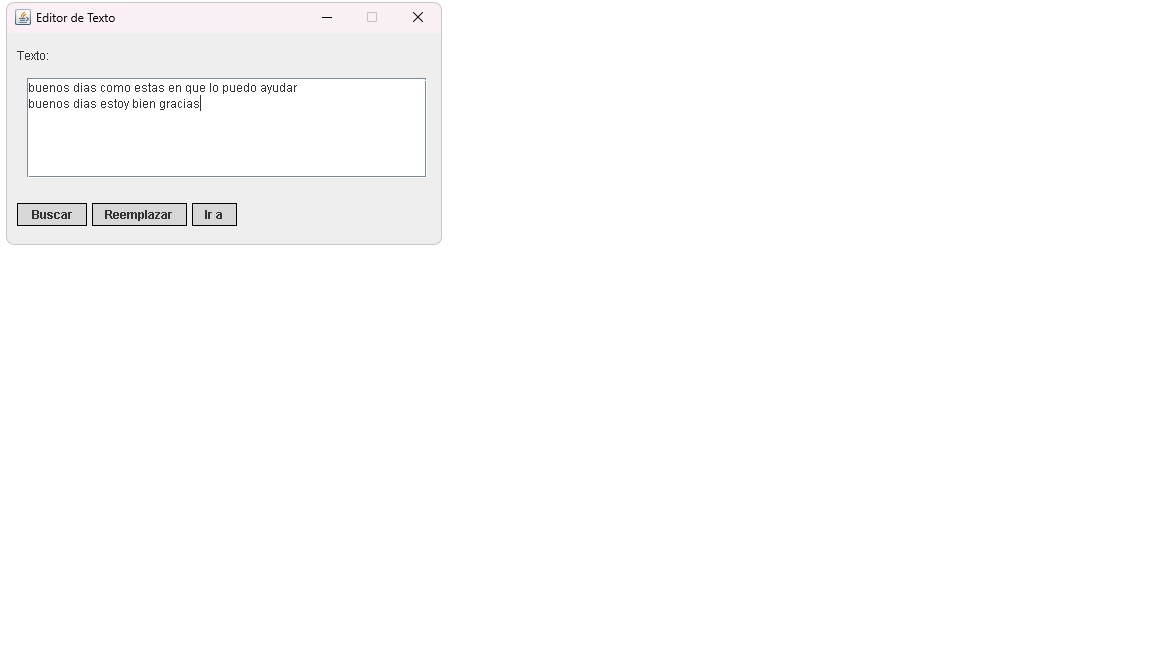
\includegraphics[width=2.5\textwidth,keepaspectratio]{img/GUI.jpg}
    \end{figure}
	\begin{figure}[H]
        \centering
		Ventana desplegable presionando el botón "buscar".
        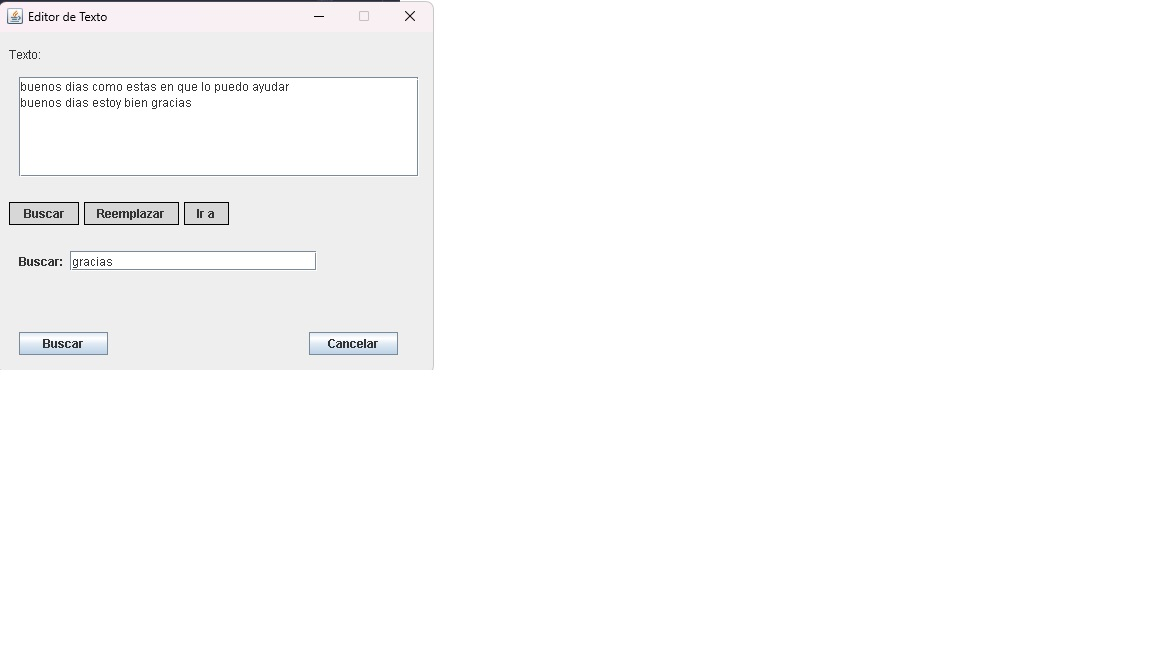
\includegraphics[width=2.5\textwidth,keepaspectratio]{img/buscar1.jpg}
    \end{figure}
	\begin{figure}[H]
        \centering
		Cuadro de aviso avisando que la palabra fue encontrada.
        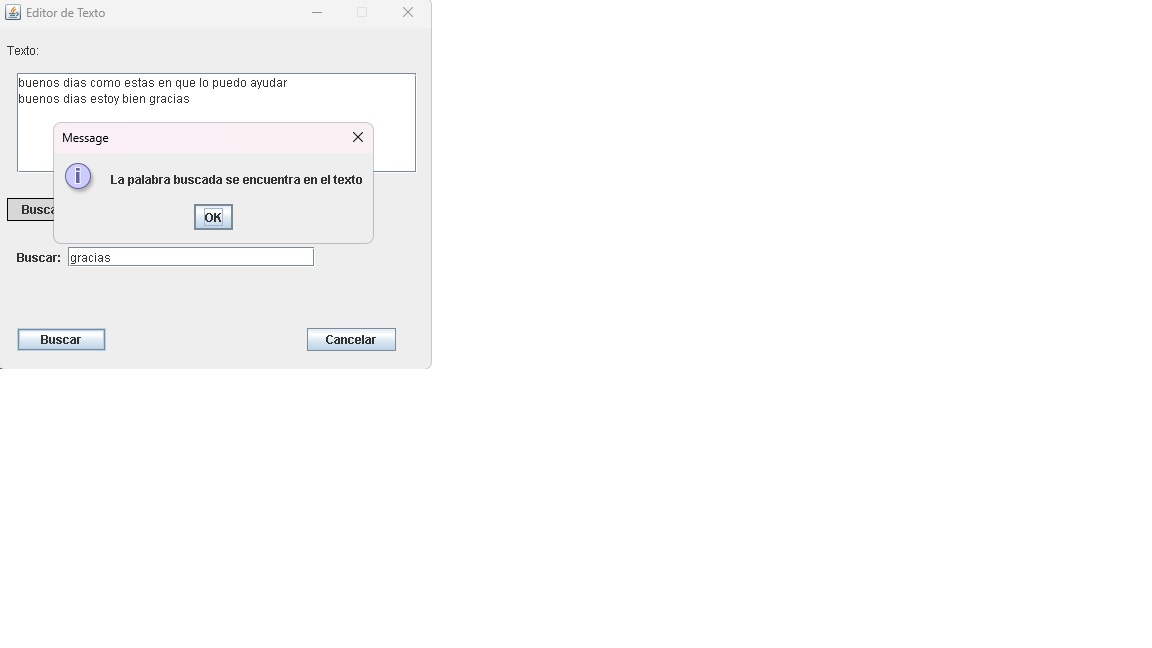
\includegraphics[width=2.5\textwidth,keepaspectratio]{img/buscar2.jpg}
    \end{figure}
	\begin{figure}[H]
        \centering
		Ventana desplegable presionando el botón "reemplazar".
        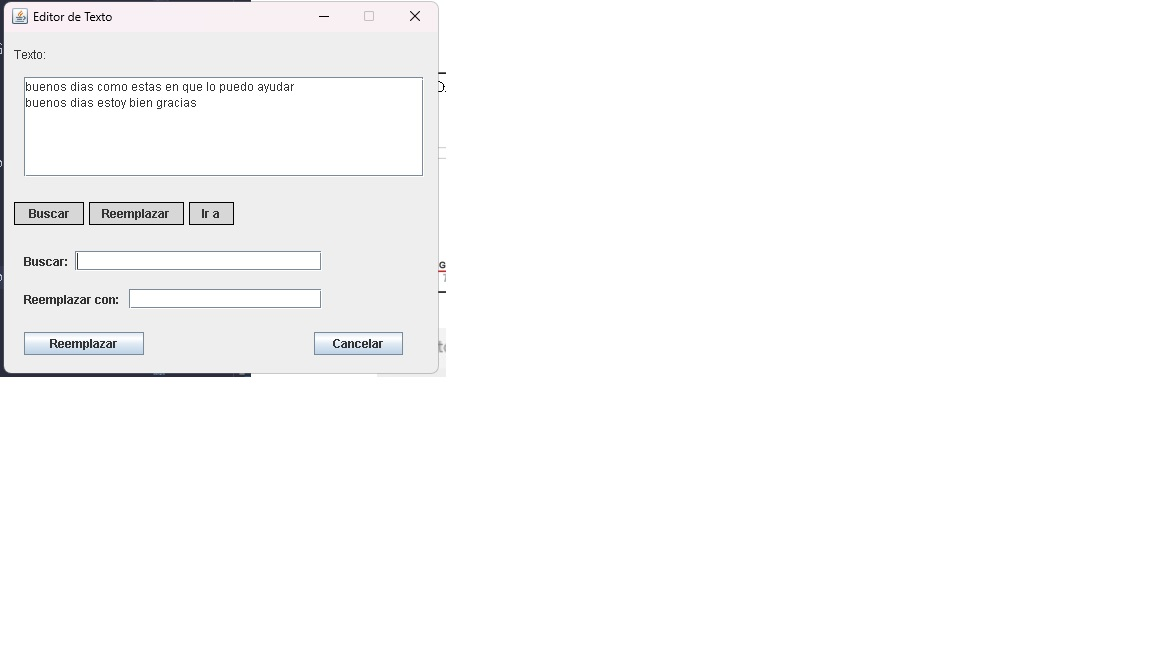
\includegraphics[width=2.5\textwidth,keepaspectratio]{img/reemplazar1.jpg}
    \end{figure}
	\begin{figure}[H]
        \centering
		Insertando texto a buscar y palabra con la cual reemplazar.
        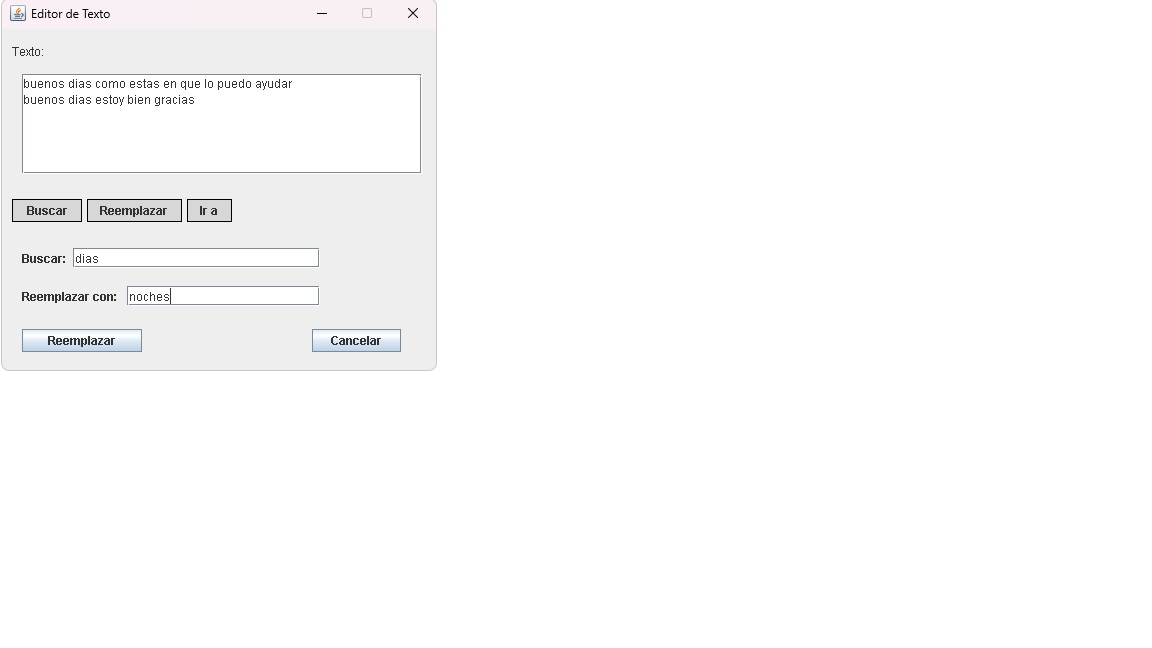
\includegraphics[width=2.5\textwidth,keepaspectratio]{img/reemplazar2.jpg}
    \end{figure}
	\begin{figure}[H]
        \centering
		Texto reemplazado.
        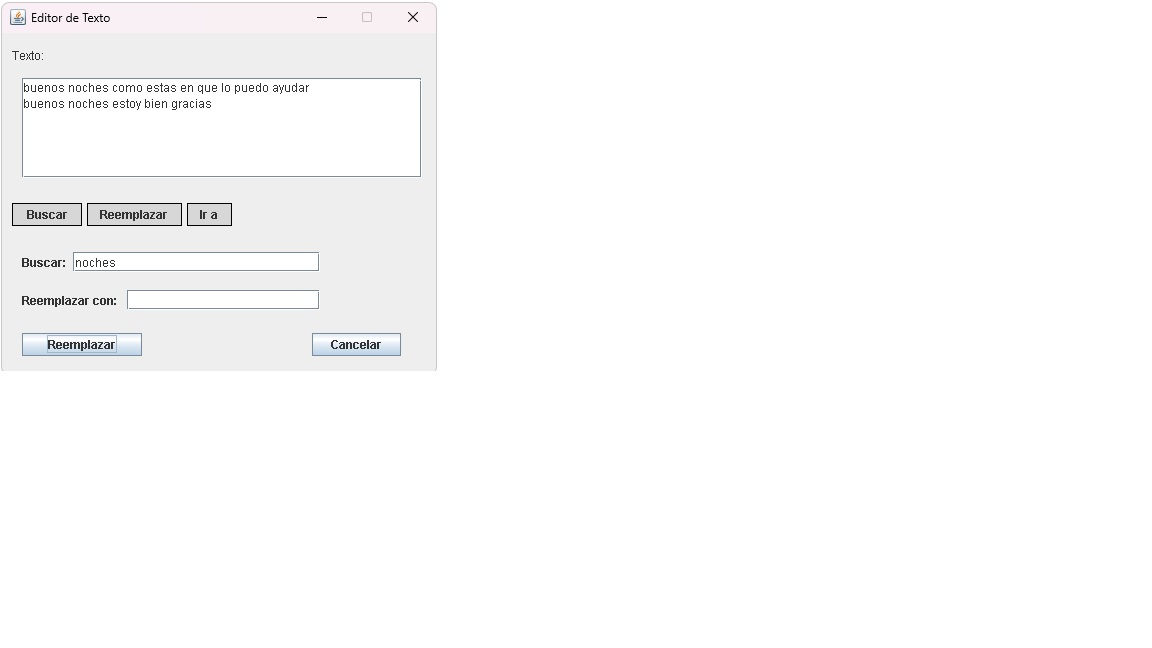
\includegraphics[width=2.5\textwidth,keepaspectratio]{img/reemplazar3.jpg}
    \end{figure}
	
	
\begin{lstlisting}[style=ascii-tree]
        
\end{lstlisting}  

\section{Cuestionario}
\subsection{Pregunta: Explique. ¿Cómo se utiliza esta estructura de datos para almacenar prefijos?.}
	\begin{itemize}
	\item  	Para almacenar prefijos, una estructura de datos comúnmente utilizada es el árbol Trie, Trie es una estructura de datos jerárquica que se organiza como un árbol en el que cada nodo representa un carácter individual de las cadenas. Los nodos en el árbol se organizan de manera que los prefijos comunes comparten los mismos nodos en la estructura, lo que lo hace muy útil para almacenar y buscar conjuntos grandes de palabras con prefijos comunes. Para almacenar prefijos usamos: inserción de una palabra, búsqueda de prefijos y eliminación.

El Trie es especialmente útil para problemas relacionados con la búsqueda y recuperación de palabras y prefijos, como la implementación de autocompletado en un motor de búsqueda o el procesamiento de diccionarios. Sin embargo, debe tenerse en cuenta que el consumo de memoria puede ser una preocupación si el Trie es extremadamente grande, ya que puede requerir mucho espacio para almacenar todas las combinaciones de caracteres posibles.

	
	\end{itemize}
	\subsection{Pregunta: ¿Cómo realizó la funcionalidad de reemplazar texto?}
	\begin{itemize}
	\item Realizamos la fucionalidad aplicando los métodos que anteriormente hemos implementado, primero con
	search() se busco las cooincidencias, despues con delete() se eliminaron y se insertaron en su posición con insert
	la nueva palabra.  	

	
	\end{itemize}		
	
	\section{\textcolor{red}{Rúbricas}}
	
	\subsection{\textcolor{red}{Entregable Informe}}
	\begin{table}[H]
		\caption{Tipo de Informe}
		\setlength{\tabcolsep}{0.5em} % for the horizontal padding
		{\renewcommand{\arraystretch}{1.5}% for the vertical padding
		\begin{tabular}{|p{3cm}|p{12cm}|}
			\hline
			\multicolumn{2}{|c|}{\textbf{\textcolor{red}{Informe}}}  \\
			\hline 
			\textbf{\textcolor{red}{Latex}} & \textcolor{blue}{El informe está en formato PDF desde Latex,  con un formato limpio (buena presentación) y facil de leer.}   \\ 
			\hline 
			
			
		\end{tabular}
	}
	\end{table}
	
	\clearpage
	
	\subsection{\textcolor{red}{Rúbrica para el contenido del Informe y demostración}}
	\begin{itemize}			
		\item El alumno debe marcar o dejar en blanco en celdas de la columna \textbf{Checklist} si cumplio con el ítem correspondiente.
		\item Si un alumno supera la fecha de entrega,  su calificación será sobre la nota mínima aprobada, siempre y cuando cumpla con todos lo items.
		\item El alumno debe autocalificarse en la columna \textbf{Estudiante} de acuerdo a la siguiente tabla:
	
		\begin{table}[ht]
			\caption{Niveles de desempeño}
			\begin{center}
			\begin{tabular}{ccccc}
    			\hline
    			 & \multicolumn{4}{c}{Nivel}\\
    			\cline{1-5}
    			\textbf{Puntos} & Insatisfactorio 25\%& En Proceso 50\% & Satisfactorio 75\% & Sobresaliente 100\%\\
    			\textbf{2.0}&0.5&1.0&1.5&2.0\\
    			\textbf{4.0}&1.0&2.0&3.0&4.0\\
    		\hline
			\end{tabular}
		\end{center}
	\end{table}	
	
	\end{itemize}
	
	\begin{table}[H]
		\caption{Rúbrica para contenido del Informe y demostración}
		\setlength{\tabcolsep}{0.5em} % for the horizontal padding
		{\renewcommand{\arraystretch}{1.5}% for the vertical padding
		%\begin{center}
		\begin{tabular}{|p{2.7cm}|p{7cm}|x{1.3cm}|p{1.2cm}|p{1.5cm}|p{1.1cm}|}
			\hline
    		\multicolumn{2}{|c|}{Contenido y demostración} & Puntos & Checklist & Estudiante & Profesor\\
			\hline
			\textbf{1. GitHub} & Hay enlace URL activo del directorio para el  laboratorio hacia su repositorio GitHub con código fuente terminado y fácil de revisar. &2 &X & & \\ 
			\hline
			\textbf{2. Commits} &  Hay capturas de pantalla de los commits más importantes con sus explicaciones detalladas. (El profesor puede preguntar para refrendar calificación). &4 &X & & \\ 
			\hline 
			\textbf{3. Código fuente} &  Hay porciones de código fuente importantes con numeración y explicaciones detalladas de sus funciones. &2 &X & & \\ 
			\hline 
			\textbf{4. Ejecución} & Se incluyen ejecuciones/pruebas del código fuente  explicadas gradualmente. &2 &X & & \\ 
			\hline			
			\textbf{5. Pregunta} & Se responde con completitud a la pregunta formulada en la tarea.  (El profesor puede preguntar para refrendar calificación).  &2 &X & & \\ 
			\hline	
			\textbf{6. Fechas} & Las fechas de modificación del código fuente estan dentro de los plazos de fecha de entrega establecidos. &2 &X & & \\ 
			\hline 
			\textbf{7. Ortografía} & El documento no muestra errores ortográficos. &2 &X & & \\ 
			\hline 
			\textbf{8. Madurez} & El Informe muestra de manera general una evolución de la madurez del código fuente,  explicaciones puntuales pero precisas y un acabado impecable.   (El profesor puede preguntar para refrendar calificación).  &4 & & & \\ 
			\hline
			\multicolumn{2}{|c|}{\textbf{Total}} &20 & & & \\ 
			\hline
		\end{tabular}
		%\end{center}
		%\label{tab:multicol}
		}
	\end{table}
	
\clearpage

\section{Referencias}
\begin{itemize}			
	\item Presentación TRIE hecha en clase por la Dra. Karim Guevara Puente de la Vega
	\item \url{https://www.youtube.com/watch?v=m9zawMC6QAI&ab_channel=ApnaCollege}
	\item \url{https://www.educba.com/trie-data-structure-in-java/}
\end{itemize}	
	
%\clearpage
%\bibliographystyle{apalike}
%\bibliographystyle{IEEEtranN}
%\bibliography{bibliography}
			
\end{document}
